\documentclass[12pt,a4paper]{article}
\usepackage[utf8]{inputenc}
\usepackage[russian]{babel}
\usepackage[OT1]{fontenc}
\usepackage{graphicx}
\usepackage{calc}
\usepackage[margin=15mm]{geometry}
\usepackage{cmap}

% условие без картинки
\newcommand{\task}[2]{
\hrule
\hbox to \textwidth {%
     \vrule
\parbox[t]{0.04\textwidth}{\smallskip \centering #1}%
     \vrule%
\hfill%
     \parbox[t]{0.93\textwidth}{\smallskip #2 \smallskip}\hfill%
\vrule
}
\hrule
    \pagebreak[2]
}

\newlength{\h}
\newsavebox{\taskbox}
\newlength{\x}
\newsavebox{\pictbox}

% условие с картинкой (картинка выравнивается по центру)
\newcommand{\taskpic}[3]{
\savebox{\taskbox}{\parbox[t]{0.93\textwidth-4.3cm}{\smallskip #2 \smallskip}}
\savebox{\pictbox}{\parbox[t]{4cm}{\smallskip \centering
     \vspace{0pt} #3 \smallskip}}
\h=\ht\taskbox
\advance\h\dp\taskbox
\x=\ht\pictbox
\advance\x\dp\pictbox
\hrule
\hbox to \textwidth {%
\vrule\parbox[t][\maxof{\h}{\x}][t]{0.04\textwidth}{ \smallskip
     \centering #1 }\vrule%
\hfill\parbox[t][\maxof{\h}{\x}][t]{0.93\textwidth-4.3cm}{\smallskip #2
     \smallskip}\hfill\vrule%
\hfill\parbox[t][\maxof{\h}{\x}][c]{4cm}{\hfil #3 \hfil}\hfill\vrule
}
\hrule
\pagebreak[2]
}
\pagestyle{empty}
\graphicspath{ {images/} }

\begin{document}
\begin{center}
\begin{Large}
\textsc{ГЦФО. 9 класс. 2014/15.}
\end{Large}
\end{center}

\taskpic{1}{В вагоне, движущемся равноускоренно по прямым горизонтальным рельсам, экспериментатор фотографировал упругий шарик, отскакивающий от пола. При этом он отпускал шарик без начальной скорости (относительно вагона) с некоторой фиксированной высоты. Фотоаппарат был неподвижен относительно вагона, плоскость траектории шарика лежала в плоскости снимка. В результате экспериментатор получил изображение траектории шарика между первым и вторым отскоками (см. рис.). Найдите ускорение вагона. Чему равно расстояние между первой и второй точками касания шариками пола, если время между отскоками равно $\tau=0{,}4$~с? Постоянная $g=9{,}8$~м/с$^2$.}{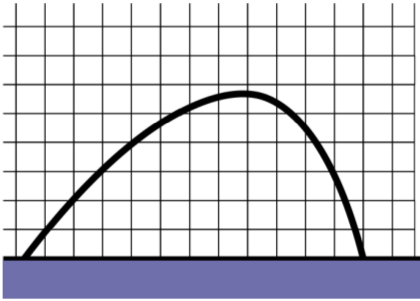
\includegraphics[width=4cm]{1}}
\taskpic{2}{Мальчик Илья играет в хитрый гольф. Ему необходимо попасть в лунку, помеченную флажком, так, чтобы мяч отскочил от очень массивной стенки и не коснулся во время своего движения земли. Стенка приближается к Илье с постоянной скоростью $u$. Илья бьет по мячу так, что начальная вертикальная составляющая скорости мяча равна $v_{\mbox{в}}$. Определите, под каким углом должен изначально полететь мяч, чтобы он попал в лунку и все правила игры были выполнены. В момент удара по мячу расстояние от стенки до Ильи $L_1$, от Ильи до лунки $L_2$.}{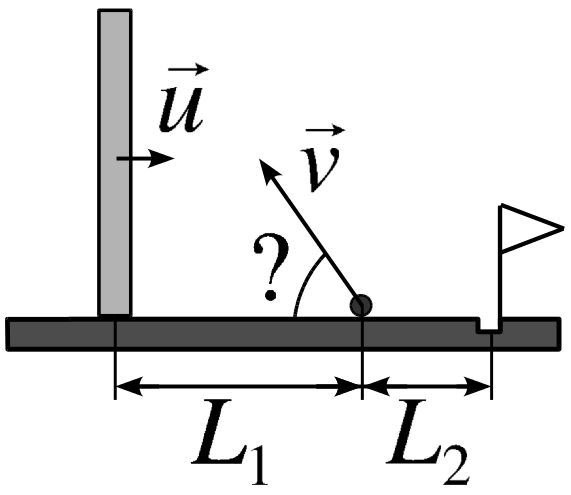
\includegraphics[width=4cm]{2}}
\taskpic{3}{На расстоянии $L=2$~м от кошки сидели мышка и лягушка. Кошка прыгнула так, чтобы поймать их за раз, в этот момент мышь начала убегать, двигаясь по прямой с постоянной скоростью, а лягушка подпрыгнула вертикально с начальной скоростью $U=4$~м/с (см. рис.). Кошка поймала лягушку на лету, а мышку --- при приземлении. Известно, что мышь была поймана через 0{,}8~с после старта. Модуль начальной скорости кошки равен 5~м/с. Найдите скорость мышки и синус угла, под которым прыгнула кошка. Ускорение свободного падения считать равным $g=10$~м/с$^2$. Всех животных считать материальными точками, которые двигаются в одной плоскости. Сопротивлением воздуха пренебречь, пойманная лягушка не влияет на траекторию кошки.}{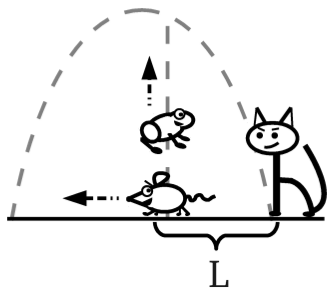
\includegraphics[width=4cm]{3}}
\task{4}{По круговой дорожке радиуса $R=40$~м одновременно стартовали два бегуна. Первый пробегает круг за 20 секунд, а второй --- за 30. Спортсмены бегут по кругу в одну сторону. Через какое время после старта относительная скорость бегунов станет максимальной? Постройте приблизительный график расстояния между бегунами по прямой от времени.}
\taskpic{5}{В солдата, сидящего в окопе, неприятель выстрелил из мортиры (см. рис.). Снаряд летел ровно на него, но до окопа не долетел. С точки зрения солдата снаряд поднимался в течение $t_1$ секунд, а опускался быстрее, за $t_2$ секунд, смотрел он из окопа от уровня земли. Известно, что неприятельские мортиры стреляют под углом $\alpha$ к горизонту, а модуль начальной скорости снаряда равен $V_0$. Найдите, на каком расстоянии от окопа упал снаряд. Сопротивлением воздуха пренебречь, ускорение свободного падения равно $g$.}{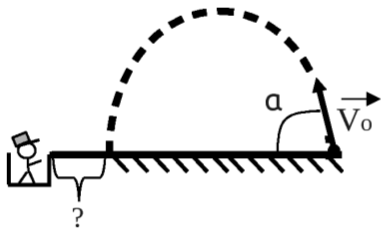
\includegraphics[width=4cm]{5}}
\taskpic{6}{Наклонная плоскость образует угол $\alpha$ с горизонтом. С высоты $H$ на нее падает мячик. Считая удары мячика о плоскость абсолютно упругими, определите расстояние между точками $n$-го и $(n+1)$-го отскока мячика от плоскости.}{
\begin{tikzpicture}[scale=0.7]
\draw[thick] (0,2)--(4,0);
\draw[thick] (0.5,2.5) node[circle,fill=black,inner sep=0,minimum size=0.1cm] {} --(0.5,1.75) node[near start,left] {$H$} parabola bend (1,2.2) (1.8,1.1) parabola bend (2.5,1.5) (3.5,0.25);
\draw[thick,dashed] (3.8,0.1)--(2,0.1);
\draw[thick] (2.8,0.1) arc (180:153.5:1) node[midway,left] {$\alpha$};
\end{tikzpicture}
}
\taskpic{7}{Тело соскальзывает с гладкой горки с высоты $H$. Отрыв тела от горки происходит на высоте $h$, при этом скорость тела горизонтальна. При каком значении $h$ дальность полета тела будет максимальной?}{
\begin{tikzpicture}[scale=0.7]
\draw[thick] (1,3)--(0,3)--(0,0)--(4,0)--(4,1) node[midway,right] {?};
\draw[thick] (4,1) parabola (1,3);
\draw[thick,dashed] (1,3.1) parabola[bend at end] (4,1.1) parabola (5.5,0);
\draw[thick,<->] (0.5,0)--(0.5,3) node[midway,right] {$H$};
\end{tikzpicture}
}
\taskpic{8}{Для создания зловещего механизма Мегамозг вскрыл тайное хранилище, содержащее три резистора с сопротивлениями 1~Ом, 4~Ом и 5~Ом. Однако из-за происков врагов надписи на резисторах оказались стерты. Тогда Мегамозг собрал из них верхнюю схему, изображенную на рисунке, и подключил к ней батарейку напряжением 1,2 B. Амперметр показал ток 0,5 А. Затем он собрал нижнюю схему, и, когда он подключил эту схему к батарейке, амперметр сгорел. Однако мастер злодейства не расстроился, ведь теперь он знал, где какое сопротивление. Чему равны сопротивления $R_1$, $R_2$, $R_3$? Амперметр сгорает, если через него течет ток больше 1 А. }{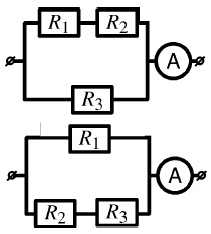
\includegraphics[width=4cm]{8}}
\taskpic{9}{Две прямые, пересекающиеся под углом $\alpha$, движутся перпендикулярно самим себе со скоростями $v_1$ и $v_2$.  Определите скорость $v$ точки пересечения прямых.}{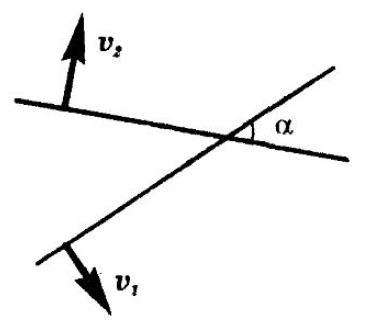
\includegraphics[width=3cm]{9}}
\taskpic{10}{Чиполлино решил сделать святящуюся эмблему своего любимого футбольного клуба <<Зенит>>. Он собрал электрическую схему, как показано на рисунке. Все буквы он составил из неоновых лампочек с одинаковым сопротивлением $R$ (на рисунке толстые черные линии между серыми точками) и соединил их проводами (сопротивление которых пренебрежимо мало, на рисунке тонкие линии). Лампа начинает светиться, если через нее течет сколь угодно малый ток. Нарисуйте, как выглядела светящаяся часть названия клуба, когда Чиполлино подключил напряжение к клеммам 1 и 2. Ответ поясните.}{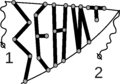
\includegraphics[width=4cm]{10}}
\task{11}{Два одинаковых вольтметра соединили параллельно, третий вольтметр подключили к этой комбинации последовательно, и к концам получившейся цепи присоединили идеальную батарейку. При этом вольтметры показывают 4 В, 4 В и 5 В. Какое напряжение у батарейки? Могут ли быть одинаковыми все три вольтметра? Что покажут эти же приборы, если их все соединить последовательно и подключить к той же батарейке? Показания приборов считайте точными.}
\taskpic{14}{B системе, изображенной на рисунке, пружины имеют жесткости $k_1=1
\begin{tikzpicture}[scale=0.8]
\draw[thick,interface] (0,5)--(2.5,5);
\draw[thick] (0.5,5)--(0.5,4.5);
\draw[spring] (0.5,4.5)--(0.5,3.5) node[midway,left] {$k_1$};
\draw[thick] (0.5,3.5)--(0.5,3);
\draw[thick] (1,3) circle [radius=0.5];
\draw[thick] (1.5,3)--(1.5,5);
\draw[thick] (1,3)--(1,1.5);
\draw[thick] (1.5,1.5) circle [radius=0.5];
\draw[thick] (2,1.5)--(2,3.5);
\draw[spring] (2,4.5)--(2,3.5) node[midway,right] {$k_2$};
\draw[thick] (2,4.5)--(2,5);
\draw[thick] (1.5,1.5)--(1.5,0.5);
\filldraw[thick,fill=gray] (1,0.5) rectangle (2,0) node[right] {$M$};
\end{tikzpicture}
}
\end{document}
